\documentclass[11pt]{article}
\usepackage[utf8]{inputenc}
\usepackage{graphicx}
\usepackage{enumitem}
\usepackage[margin=0.3in]{geometry}
\usepackage[dvipsnames]{xcolor}
\usepackage{yfonts}

\usepackage{aurical}
\usepackage[T1]{fontenc}
\usepackage{tabularx}
\usepackage{watermark}
\usepackage{MnSymbol}
\usepackage{tikz}
\newcommand*\circled[1]{\tikz[baseline=(char.base)]{
            \node[shape=circle,draw,inner sep=2pt] (char) {#1};}}
\definecolor{OCRA}{RGB}{204,119,34}

\begin{document}
\thiswatermark{\centering \put(-50,-850){
\includegraphics[scale=1.5]{img/paper.jpg}} }
\begin{minipage}{0.4\textwidth}
    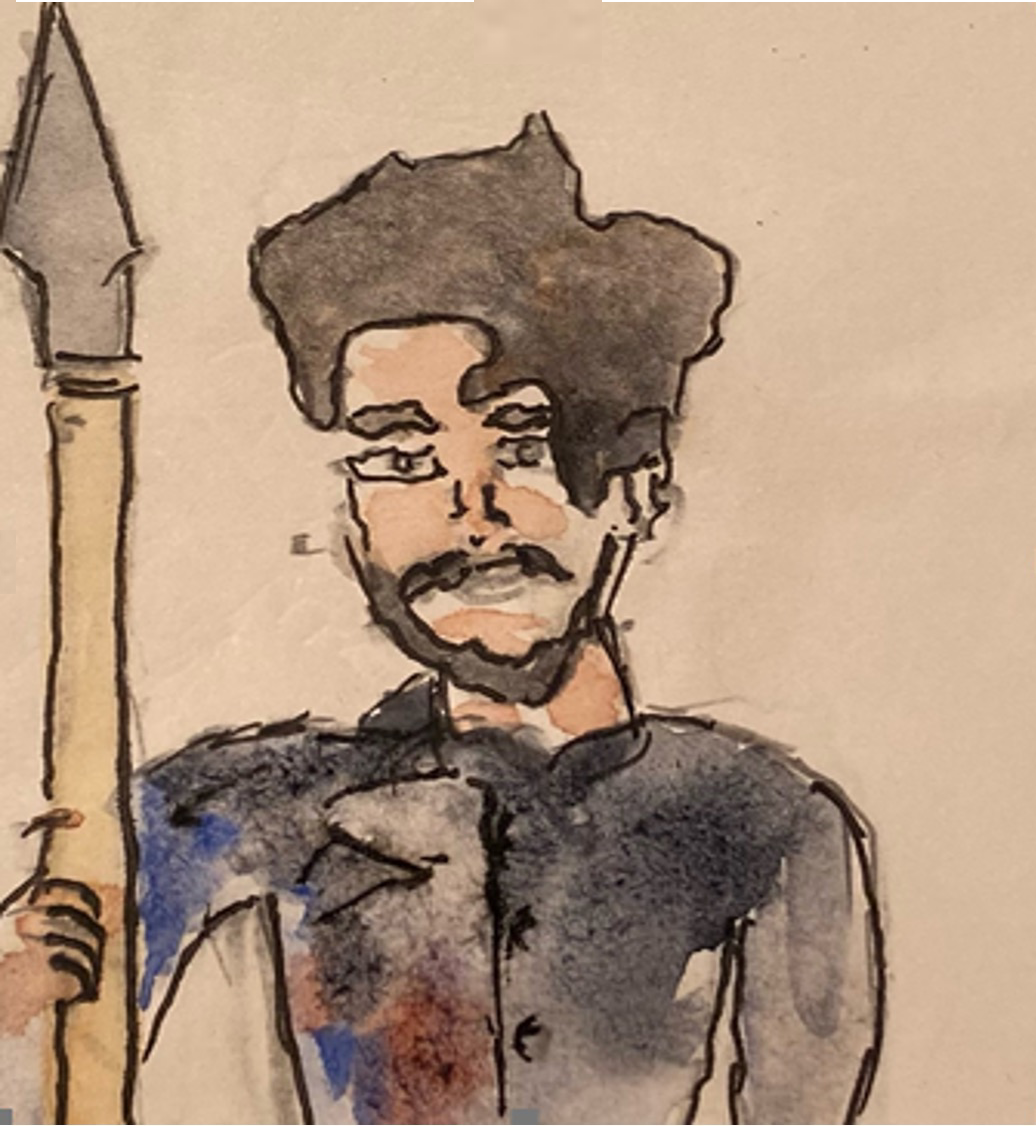
\includegraphics[scale=0.45]{img/arnosto.png}
\end{minipage}%
\hspace{0.4cm}
\begin{minipage}{0.55\textwidth}%\raggedleft
    \Huge{\Fontauri The Real Arnosto} \\
    \Large{Fighter 2/Magic User 2} \\
    \begin{normalsize}
        \begin{itemize}[topsep=0pt, itemsep=0pt, partopsep=0pt, parsep=0pt, leftmargin=*]
            \item Is about 5’ tall has bushy black hair has a beard that keeps growing back, no matter how often he shaves
            \item has bare feet, which is not uncommon in these parts
            \item has hazel eyes
            \item sports a minimal smile, in fact it is probably a quarter of a smirk; the only way to tell if he is happy is if you can see a sparkle in his eyes
        \end{itemize}
    \end{normalsize}
    \begin{large}
        \vspace{0.4cm}
        \begin{tabular}{cccccc}
            Str & Int & Wis & Dex & Con & Cha \\ \hline
            13 & 11 & 8 & 11 & 11 & 10\\ 
            $\ostar$ & & & & & 
        \end{tabular}
    \end{large}
    \vspace{0.4cm}

    \begin{minipage}[t]{0.2\textwidth}
        \begin{large}
            \begin{tabular}[t]{lc}
                \textcolor{OCRA}{HP} & \circled{12}\\
                \textcolor{OCRA}{AC Leather} & \circled{\ 7}
            \end{tabular}
        \end{large}
    \end{minipage}
    \hspace{1.0cm}
    \begin{minipage}[t]{0.2\textwidth}
        \begin{large}
            \begin{tabular}[t]{lc}
                \textcolor{OCRA}{AC Mail} & \circled{\ 5}\\
                \textcolor{OCRA}{AC Plate} & \circled{\ 3}
            \end{tabular}
        \end{large}
    \end{minipage}
    \hspace{1.0cm}
    \begin{minipage}[t]{0.2\textwidth}
        \begin{large}
            \begin{tabular}[t]{lc}
                \textcolor{OCRA}{Shield} & \circled{-1}
            \end{tabular}
        \end{large}
    \end{minipage}
\end{minipage}
 
 \vspace{0.5cm}
 \begin{quote}
 \textit{\Fontauri"Un giovane kenku che ha passato la vita da una stiva della nave e l'altra. Utilizzato fin da piccolo come sguattero, alternava il lavoro all'ascoltare i canti di mare dei marinai che ripeteva poi alla perfezione. Questo lo rese molto desiderato da varie ciurme, in quanto poteva allietare con i suoi canti le lunghe notti in mare. Viene infine comprato dal mercante Mimuda, contrabbandiere semi ufficiale di perle. La ciurma di Mimuda compra perle illegalmente nelle paludi di Uada e le rivende a Fedris. Il suo ruole e inizialmente di semplice messaggero, ma con il passare degli anni diventa l'uomo piu fidato del ricco mercante. Zitto vive vari anni al servizio del suo benefattore, fino a quando non viene a scoprire un suo terribile segreto. Infatti Mimuda sfruttava gli effetti di perdita di memoria delle paludi di Uada per uccidere membri scomodi delle sua ciurma, senza che i restanti si ricordassero di nulla. Una frase scomoda, ripetura a pappagallo, nel momento sbagliato lo inserisce nella lista nera di Mimuda e lo costringe alla clandestinita per sfuggire alla carneficina.  "}  
 \end{quote}

\begin{minipage}[t]{.5\textwidth}
{\huge \Fontauri Features}\\
\textcolor{OCRA}{Kenku}\\
\textbf{Mimica} Puoi riprodurre i suoni che hai sentito, incluse le voci.\\
\textbf{Contraffazione Esperta} Puoi duplicare manufatti e scritture di altre creature. Disponi di vantaggio \\
\textcolor{OCRA}{Bard}\\
\textbf{Bardic Inspiration}(d8)\\
\textbf{Jack of all trades} Half Proficiency to Ability Check\\
\textbf{Song of Rest} 1d6 to Short Rest\\
\textbf{Font of ispiration} BI regained with Short Rest\\
\textbf{Countercharm} As an action start to sing. All allies in 30f have adv on being charmed or frightened.\\
\textcolor{OCRA}{College of Lore}\\
\textbf{Cutting Words} When a creatures make an attack roll 60f from you you can use a BI and sub from the attack.\\
\textbf{Additional Magic Secrets}\\
\textcolor{OCRA}{Rouge}\\
\textbf{Cunning Action}\\
\textbf{Sneak Attack (1d6)}\\
\end{minipage}
\begin{minipage}[t]{.4\textwidth}\raggedleft
\begin{center}
{\Huge \textgoth{P}} \circled{\Huge +4} \hspace{0.3cm} {\Huge \textgoth{A}} \circled{\Huge+8} \hspace{0.3cm} {\Huge \textgoth{S}} \circled{\Huge+9} {\Huge \textgoth{Q}} \circled{\Huge+2}
\end{center}

\vspace{0.5cm}
{\Large \textbf{\Fontauri Skills}}\\
Athletics $\bullet$\\
Acrobatics \\ 
Deception $\bullet$\\ 
Investigation \\
Perception $\bullet$ \\
Performance $\bullet$\\ 
Stealth $\bullet$ \\

\vspace{.5cm}

{\Large \textbf{\Fontauri Sailor Background}}\\
A belaying pin(club)\\
50 feet of silk rope\\
A gemstone (coal for others)\\

\vspace{0.5cm}

{\Large \textbf{ \Fontauri Tools}}\\
Navigator's tools\\
vehicle(water)\\


\end{minipage}

\newpage
\thiswatermark{\centering \put(-50,-850){
\includegraphics[scale=1.5]{img/paper.jpg}} }

\begin{minipage}[t]{.5\textwidth}
{\huge \textbf{\Fontauri Spells}}\\
\textcolor{OCRA}{Cantrips}\\
Mending\\
Message\\
Vicious Mockery\\
\textcolor{OCRA}{1th Level (4)}\\
Bane \\
Charm Person\\
Detect Magic\\
Protection from Evil and Good\\
\textcolor{OCRA}{2nd Level (3)}\\
Invisibility\\
Shatter\\
Enthrall\\
Gift of Gab\\
\textcolor{OCRA}{3rd Level (3)}\\
Fly\\
Haste\\
Fireball\\
Hypnotic Pattern\\
Stinking Cloud\\
Wind Wall\\
\textcolor{OCRA}{4th Level (2)}\\
Stone Shape\\
Wall of Fire\\
Hallucinatory Terrain\\
Animate Objects
\end{minipage}
%CONTINUE OF EQUIPMENT
\begin{minipage}[t]{.4\textwidth}\raggedleft
{\Large \textbf{ \Fontauri Equipment}}\\
Magic Gun \\
Entertainers pack\\
Cli Lyre\\ - Broom of flying - Cap of Waterbreathing\\
Leather armor \\
Dagger\\
Thieves tools\\
Slippers of spider climbing\\

\end{minipage}
\end{document}
